\documentclass[a4paper,11pt]{article}

% set up sensible margins (same as for cssethesis)
\usepackage[paper=a4paper,left=30mm,right=30mm,top=25mm,bottom=25mm]{geometry}
\usepackage{natbib} % Use the natbib bibliography and citation package
\usepackage{setspace} % This is used in the title page
\usepackage{graphicx} % This is used to load the crest in the title page

% non-template packages
\usepackage{paralist}
\usepackage{multicol}
\usepackage{caption}
\usepackage{tabularx, booktabs}
\newcolumntype{Y}{>{\centering\arraybackslash}X}


\usepackage{hyperref}
\usepackage{xcolor}
\usepackage{lscape}
\hypersetup{
	colorlinks,
	linkcolor=teal,
	citecolor=teal,
	urlcolor=blue
}

%tikz stuff
\usepackage{tikz}
\usetikzlibrary{shapes, arrows, trees}
\tikzstyle{decision} = [diamond, draw, fill=green!20, text width=4.5em, text badly centered, node distance=3cm, inner sep=0pt]
\tikzstyle{block} = [rectangle, draw, fill=yellow!20, text width=3cm, text centered, rounded corners, minimum height=4em]
\tikzstyle{line} = [draw, -latex']
\tikzstyle{straight} = [draw]


\usepackage{array}
\newcolumntype{L}[1]{>{\raggedright\let\newline\\\arraybackslash\hspace{0pt}}m{#1}}
\newcolumntype{C}[1]{>{\centering\let\newline\\\arraybackslash\hspace{0pt}}m{#1}}
\newcolumntype{R}[1]{>{\raggedleft\let\newline\\\arraybackslash\hspace{0pt}}m{#1}}


%\hypersetup{
%	colorlinks,
%	linkcolor={red!50!black},
%	citecolor={blue!50!black},
%	urlcolor={blue!80!black}
%}

\begin{document}

% Set up a title page
\thispagestyle{empty} % no page number on very first page
% Use roman numerals for page numbers initially
\renewcommand{\thepage}{\roman{page}}

\begin{spacing}{1.5}
\begin{center}
{\Large \bfseries
School of Computer Science \\
Monash University}

\vspace*{30mm}


\includegraphics[width=5cm]{graphics/MonashCrest.pdf}

\vspace*{15mm}

{\large \bfseries
Research Proposal --- Comp Sci Honours, 2017
}

\vspace*{10mm}

{\LARGE \bfseries
Exploring improvements to Part-to-picker systems in Warehouses 
}

\vspace*{20mm}

{\large \bfseries
Phillip Wong 25150510

\vspace*{20mm}


%Supervisors: \parbox[t]{50mm}{Daniel Harabor}, \\Another person}
Supervisor: Daniel Harabor
}

\end{center}
\end{spacing}

\newpage

\tableofcontents

\newpage
% Now reset page number counter,and switch to arabic numerals for remaining
% page numbers 
\setcounter{page}{1}
\renewcommand{\thepage}{\arabic{page}}

	\begin{abstract} %100-200 words
	\noindent \textbf The order picking process is the number one expense in warehouse systems. Here we look at part-to-picker a type of order picking where the products are autonomously retrieved and given to the pickers. Previous research have focused on improvements in the multi-agent path finding but they often overlook simple adjustments or additions which may reduce complexity of the problem.  This project will test the effect that these aspects have on improving order-picking. We will create a simulation and focus on the warehouse layout first. The results of this project will help identify how small adjustments may increase the efficiency of the order picking process.
	
\end{abstract}
\section{Introduction}
In warehouse management, order picking is the process whereby a product is retrieved according to incoming customer orders. This process has been identified by \cite{de2007design} as the most costly process in operating a warehouse, estimated to take 55\% of the warehouse operating cost.

% cONVEYER BELTS ARE SORTING SYSTEMS NOT PART-TO-PICKER SYSTEMS A well-known example is the use of conveyor belts to move orders around. The down-side of conveyor systems are their high operational and maintenance cost as well as the rigid infrastructure needed for them to operate

Here we look at a type of order picking known as part-to-picker systems which deals with automating the movement of products from storage areas to picking stations, where workers will manually pick the orders. (\cite{wurman2008coordinating}). Part-to-picker systems often employ the use of automated vehicles when retrieve the orders from where they are stored. \cite{introduction2015autostore} is a recent system where products are organized in a grid of stacked bins. Robots move around the top of the grid, lifting bins and delivering them to a human picker. Benefits of the AutoStore system include high storage density and expansion capability. While not much literature is published about the specifics of AutoStore, we suspect some downsides of this system to be similar to conveyor belts with high operational and maintenance costs as well as high retrieval cost.

In this project we look at Kiva Systems (now known as Amazon Robotics). In Kiva systems, products are stored in shelves known as storage pods. Robots known as drive units are responsible for picking up and carrying storage pods to picking stations (see Fig \ref{kivaprocess} and \ref{kivalayout1}).
\begin{figure}[h!]
	\centering
	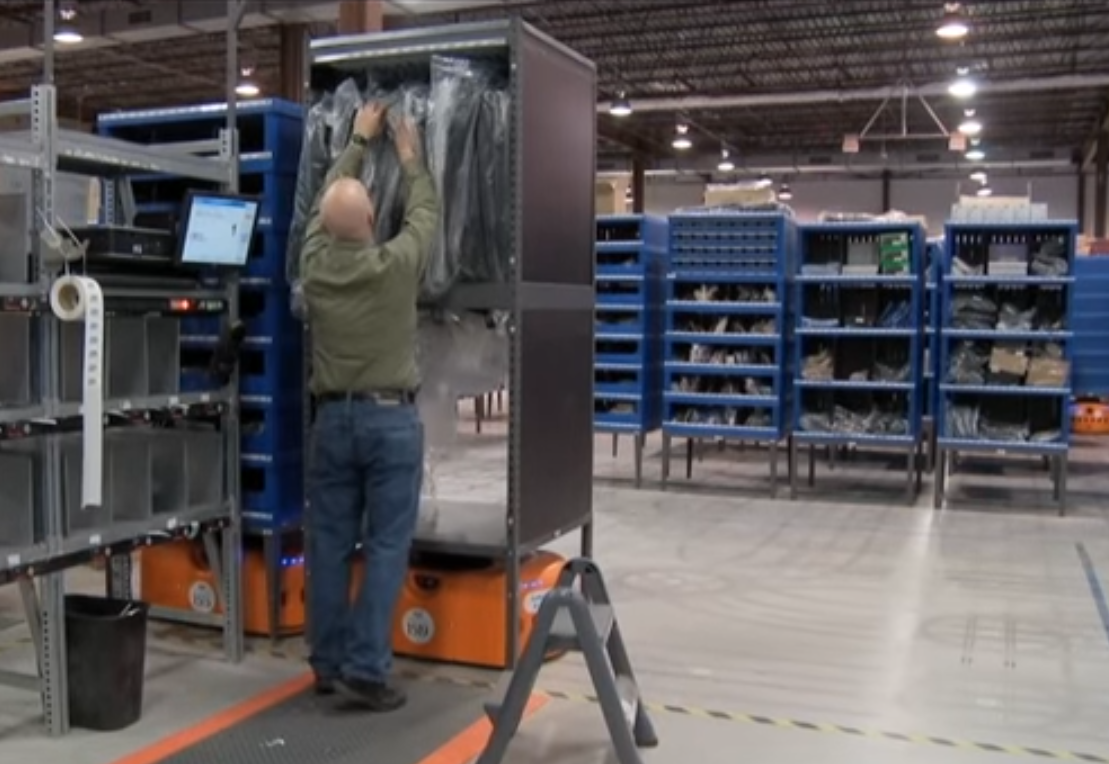
\includegraphics[width=0.8\textwidth ]{graphics/kivaprocess}
	\caption{A worker picking an order from a storage pod. The orange robot underneath is the drive unit. (\cite{kivayoutube2010quietlogistics})}
	\label{kivaprocess}
\end{figure}

\noindent The process for a drive unit is as follows:

\begin{compactenum}
	\item Unit is told to retrieve a product
	\item Unit moves to the storage pod containing the product and picks up the pod
	\item Unit carries the pod to a picking station
	\item Human worker picks the product from the pod and packs it
	\item Unit returns the pod back to where it was picked up
	\item Unit waits until it is told to retrieve another product
\end{compactenum}

\noindent Kiva systems do not require a complex infrastructure to operate hence solving issues found in alternative solutions: maintenance and operational costs. When a unit malfunctions it can be easily accessed and replaced, moreover the system remains operational. The initial setup for a warehouse is cheap and fast as a warehouse needs only storage pods, a picking station and a number of drive units to operate.

%\subsection{Need for the study}
%Cooperative Multi-agent pathfinding has historically seen a lot of research in games but recently has risen in real world usage with robotics. Some of these fields includes disaster rescue, self-driving cars and automated ports

Kiva Systems deal with a number of problems, in this project we will be focusing on the multi-agent pathfinding (MAPF) problem. MAPF aims to find a path from for each agent (drive unit) so that they can reach their goal while ensuring that no path conflicts with another. Finding an optimal solution to multi-agent pathfinding is an NP-hard problem (\cite{yu2013structure}), has applications in systems containing few agents. This is not an option as Kiva systems deal with hundreds of agents, for example the Office Supply company, Staples uses 500 robots in their 30000$m^{2}$ center (\cite{guizzo2008three}). Here we aim to reduce the number of conflicts in pathfinding by exploring a number of adjustments that can be made to the system.

\subsection{Research questions}
In order to explore the improvements that can be made to improving Kiva systems, we aim to answer two main questions:

\begin{enumerate}
	\item What adjustments can be made to Kiva systems to simplify the pathfinding?
\begin{compactitem}
	\item An improved layout of storage pods and picking stations
	\item Allowing drive units are capable of maneuvering underneath storage pods
	\item An intermediate zone for drive units to drop off storage pods
\end{compactitem}

\item How much faster will the path search run by pre-computing paths and storing them in a path oracle?

\end{enumerate}

\section{Literature Review}
\textbf{HALF-DONE} There are a number of problems in Warehouse Automation, some of these we will be looking at in this project include: multi-agent pathfinding, order sequencing and warehouse design.

In multi-agent pathfinding, \cite{cohen2016bounded} uses highways.

\cite{strasser2015compressing} uses Compressed Path Databases.

\cite{gu2010research} provides a comprehensive review of warehouse design and performance. It covers 5 major aspects, overall structure, sizing and dimensioning, department layout, equipment selection and operation strategy selection.

\cite{de2007design} provides a survey on order picking

\cite{wurman2008coordinating} provides an in depth overview of Kiva Systems, describing their benefits, usages and research areas.




\cite{ma2016optimal} presents a Conflict-Based Min-Cost-Flow algorithm which is correct, complete and optimal. It implements it on Kiva Systems looking at hundreds of agents split into dozens of teams.





%Unlike existing literature, in this project we aim looking at a number of other factors which are likely to simplify the pathfinding problem.

%Windowed Hierarchical Cooperative A∗. Cooperative A*. Conflict-Oriented Windowed Hierarchical Cooperative A∗. Compressed Path Databases.

\cite{de2007design} overview of picking

\cite{boysen2017parts} looks at the batching and sequencing of inventory orders which are given to units. Their study found that only half the units is needed when orders are optimized optimized picking allows

\section{Methodology}
\label{Research}
\subsection{Path oracle}

\cite{strasser2015compressing}


\noindent \textbf{PLACEHOLDER} Decentralised MAPF algorithms usually involve search. A typical problem solving process (e.g. FAR (Wang \& Botea, ICAPS 2008)) involves each agent finding a path independent from all the rest (i.e. if there are k agents we solve k single-agent problems separately). When all agents have a path they each take turns moving one step at a time towards their goal. Conflicts are resolved locally choosing in favour of one agent over another in some way (e.g. assign a priority to each agent and always favour the agent with highest priority). We aim to improve efficiency by introducing a path oracle which removes entirely the need to search. The oracle is pre-computed up front and reused for every subsequent pathfinding query thereafter. Since the cost of the initial path searches tends to dominate runtime in MAPF we expect this approach will significantly improve performance. \textbf{PLACEHOLDER}

\subsection{Warehouse layout}
Usually the picking station is positioned on one side of the warehouse and the pods are laid out in rows (Fig. \ref{kivalayout1}).

\begin{figure}[h]
	\centering
	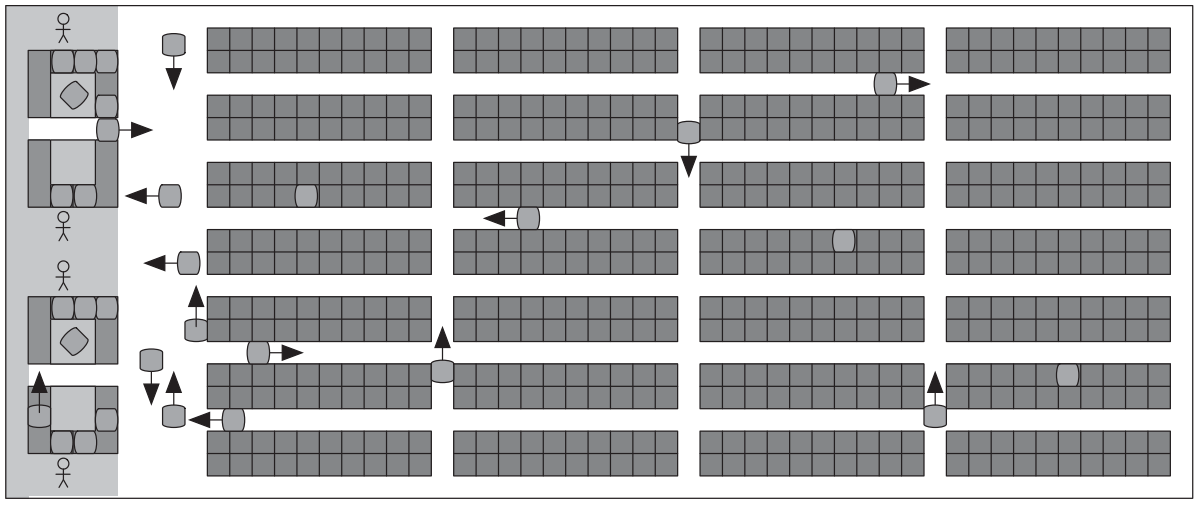
\includegraphics[width=0.9\textwidth]{graphics/kivasystemlayout}
	\caption{A Small Region of a Kiva Layout (\cite{wurman2008coordinating}). Picking stations located on the left and storage pods laid out in rows.}
	\label{kivalayout1}
\end{figure}

\cite{wilt2014spatially} looked at identifying zones by areas which are bottlenecks and assigning a controller, for that zone which manages any agents who need to travel through the bottleneck. Inspired by this and assuming pickup stations, we plan to split the warehouse into two halves and introduce an intermediate zone (See Fig \ref{kivalayout2}). Delivering pods which are situated in the far zone is a two step process:
\begin{compactenum}
	\item Units in the far zone move pods to the intermediate zone instead of a pickup station
	\item Units in the delivery zone will pickup pods in the intermediate zone
\end{compactenum}
\noindent These zones will have their own controller which handles any agents within the zone and tells them what behaviour should occur.

\begin{figure}[h]
	\centering
	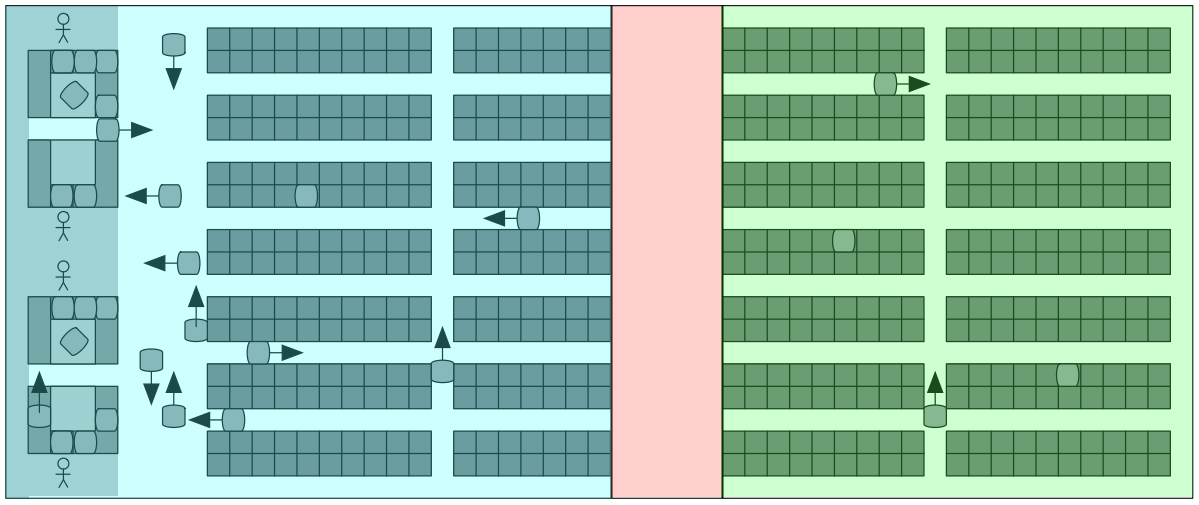
\includegraphics[width=0.9\textwidth]{graphics/kivasystemlayout_adjusted}
	\caption{Intermediate zone in red, delivery zone in blue and far zone in green}
	\label{kivalayout2}
\end{figure}

\subsection{Order picking}
As pods can be dynamically move around the warehouse, the layout pods can be changed to suit incoming orders. Storage pods containing popular orders may be placed next to a picking station so a drive unit can readily access it and unpopular orders will be placed further away. Vice-versa the distribution of orders can be re-ordered to suit the current layout of the warehouse. Here we may take inspiration from Robin-hood hashing and apply it to sorting the inventory pods. \cite{boysen2017parts} covered both of these aspects in detail and revealed that after optimizing orders, the total number of drive units can be cut by half and retain the same supply to picking stations.

% proving that the problem is NP-hard for even a single order and that their solution is strongly NP-complete.

\subsection{Allowing for movement underneath storage pods}
As drive units are capable of moving underneath pods when carrying them, this means that with small adjustments to the dimensions of storage pods it is possible to allow drive units to maneuver underneath the pods. With this the only obstacles in the environment are other drive units.

\subsection{Timetable/plan}
\textbf{HALF DONE}
\begin{center}
{\footnotesize
\begin{tabular}{ c p{12cm} }
\multicolumn{2}{l}{\textbf{Semester 1}} \\
\hline \multicolumn{1}{c}{Week(s)} & \multicolumn{1}{c}{Plan} \\
\hline 7  & Model warehouse and simple A* pathfinding \\
\hline 8  & Add multiple agents with A* assigned random pods (no picking station) arsasarsa\\
\hline 9  & Implement Cooperative A* \\
\hline 11 & Add simple scheduler which assigns agents a location to fetch a random pod and return to the picking station \\
\hline 12 & Focus on Interim Presentation \\
\hline 13 & Focus on Literature Review \\
\hline 14 & Focus on Examinations \\
\hline Holidays & Implement Path Oracle with Compressed Path Databases \\
\hline
\end{tabular}
}


{\footnotesize
\vspace{0.5cm}
\begin{tabular}{ c p{12cm} }
\multicolumn{2}{l}{\textbf{Semester 2}} \\
\hline \multicolumn{1}{c}{Week(s)} & \multicolumn{1}{c}{Plan} \\
\hline 1  & Add more complex scheduler, distributing requested inventory  and allow agents dynamically sort pods according to popularity. Agents dynamically sort pods according to popularity. Decide on the focus for the rest of the project. \\
\hline 2-4 & Implement Path Oracle with Compressed Path Databases \\
\hline 3  &  \\
\hline 4  & \\
\hline 5  &   \\
\hline 6  &  \\
\hline 7  & \\
\hline 8  & \\
\hline 9  & \\
\hline 10 & \\
\hline 11 & \\
\hline 12 & Finish Final Thesis \\
\hline 13 & Additional tasks \\
\hline 14 & Focus on Final Presentation \\
\hline 15 & Focus on Final Thesis \\
\hline
\end{tabular}
}
\end{center}


\section{Expected Outcomes}
% (Expected) outcomes of the project are discussed with appropriate level of detail, and are presented coherently to illustrate varying levels of implications and contributions the project offers. 
% (Expected) outcomes are logically and consistently aligned against the relevant research questions/aims

We suspect that these adjustments will reduce the number of conflicts in the MAPF problem hence allowing for a better bounded suboptimal solution to be found. Regardless of results, we expect to be able to better understand the explored properties described in Section \ref{Research} and their effect on Kiva systems.

Additionally we hope to deliver an improved MAPF solution utilizing a pre-computed path oracle and a simulation showcasing its usage in a Kiva system.


%\section{Glossary of terms} % Temporary, delete later

%\begin{enumerate}
%	\item avoidance
%	\item path planning
%	\item Drive Unit Agent (DUA)
%	\item Storage Pod
%	\item Makespan
%	\item Idle time
%	\item Performance curve relative to..?
%	\item Robin-hood hashing
%   \item order distribution systems
%\end{enumerate}

\bibliographystyle{dcu}
\bibliography{bibliography}


\end{document}
